%!TEX root = ../thesis.tex

\section{関連研究}
歩行者の複雑な動きを予測するために,深層学習を応用しようという研究が,近年注目を集めている.
深層学習を歩行者の軌道予測に応用した例として,Alexandreら\cite{s-lstm}は,人間の動きを学習し,未来の軌跡を予測できるLSTMモデルを提案している.この研究は,歩行者の軌道予測に着目した最も初期の深層学習モデルの一つである.Social-LSTMは,\figref{Fig:s-lstm}のように各軌跡に1つのLSTMを使用し,プーリング機構を用いて,LSTM間で情報を共有している.このシステムにより,複数の個人にわたって相互作用から生じるさまざまな非線形行動をうまく予測することに成功した.

\begin{figure}[hbtp]
     \centering
    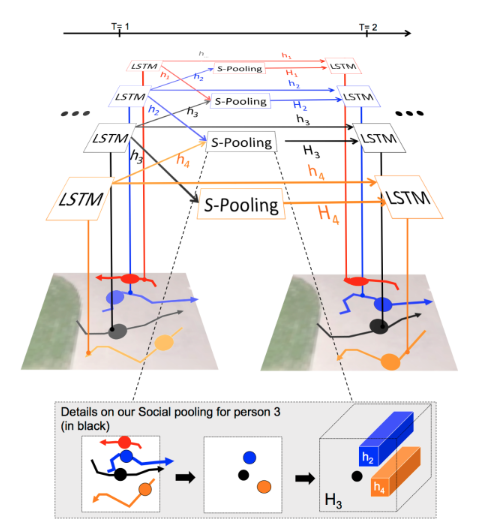
\includegraphics[keepaspectratio, scale=0.56]
         {images/s_lstm.png}
    \caption{Overview of Social-LSTM method.\protect\footnotemark[1]}
    \label{Fig:s-lstm}
\end{figure}

\protect\footnotetext[1]{\cite{s-lstm}より引用}

hogehoge

\subsection{LSTMによる歩行者の軌道予測の応用事例}
この研究では,

\subsection{GNNによる歩行者の軌道予測の応用事例}
hoge

\subsection{ロボットの将来の行動を軌道予測に用いた事例}
丹野らは,歩行者の軌道予測に過去の動きだけでなく,ロボットが選択する将来の動きを考慮して予測をしている.実験では,ロボットの将来の行動を考慮しない場合と比較して,ロボットの動きに合わせて変化する歩行者の動きを予測できている.

\subsubsection{etc...}
\newpage
